%% 美赛模板:正文部分

\documentclass[12pt]{article}  % 官方要求字号不小于 12 号,此处选择 12 号字体

% 本模板不需要填写年份,以当前电脑时间自动生成
% 请在以下的方括号中填写队伍控制号
\usepackage[2318758]{easymcm}  % 载入 EasyMCM 模板文件
\problem{C}  % 请在此处填写题号
\usepackage{mathptmx}  % 这是 Times 字体,中规中矩 
%\usepackage{mathpazo}  % 这是 COMAP 官方杂志采用的更好看的 Palatino 字体,可替代以上的 mathptmx 宏包

\title{Research on Wordle Correlation Model of Twitter\par --Based on Fitting and Cluster Analysis}  % 标题

% 如需要修改题头(默认为 MCM/ICM),请使用以下命令(此处修改为 MCM)
%\renewcommand{\contest}{MCM}
%\usepackage[UTF8]{ctex}

% 文档开始
\begin{document}

% 此处填写摘要内容
\begin{abstract}

Wordle is a puzzle game launched by the $New York Times$, which has recently become very popular on the Internet, especially on $Twitter$. In this paper, we focus on the relationship between the number of Wordle players, the proportion of choosing the difficult mode and time, and the change of word difficulty, firstly, we perform data cleaning, i.e. remove or correct the data with too much deviation, establish various fitting models in prediction, and point distribution models in word difficulty assessment, use linear fitting, non-linear fitting, and cluster analysis to solve, and calculate the final results.

For the problem of predicting the reported results on \textbf{2023/3/1} in \textbf{problem 1}, polynomial, Gaussian normal, and fractional-type functions were used to fit and calculate the correlation coefficients, and the nonlinear model with the error within the controllable range was selected for prediction, and the results were obtained as the prediction interval for the number of reported results on \textbf{2023/3/1}. For the question of determining whether the attributes of words affect the proportion of reported scores that play in the difficult mode, it is conjectured that the factors that may affect this proportion may be the number of syllables, the number of vowels, the number of repeated letters, and word frequency. A linear fit was then used to analyze whether the words used as answers the day before had a significant effect on the day after, concluding that these factors did not have a significant effect.

For \textbf{problem 2 and 3},we defined an evaluation function , which is used to calculate the difficulty score for each word, with higher difficulty scores representing easier words. Combining the main factors that affect the difficulty of words, we used K-means clustering analysis to classify the words. When we add the word '\textbf{eerie}' to one of these clusters according to its features, we can estimate its difficulty score using the scores of other words in the same cluster. This indicates that '\textbf{eerie}' has a difficulty level around 20\%, which is quite difficult. We can also predict how many attempts it will take for someone to solve '\textbf{eerie}', with 0\%, 2\%, 11\%, 32\%, 35\%, 18\% and 3\% chances of solving it in 1, 2, 3, 4, 5, 6 and X attempts respectively.

For \textbf{problem 4}, some other characteristics of the data were found using statistical analysis of the data, including fewer results reported on Sunday compared to others, a gradual increase and leveling off in the percentage of difficult patterns selected, and a higher probability of the answer words being nouns or multi-word words.

Finally, the model developed in this paper is discussed and analyzed to comprehensively evaluate the model.

    % 美赛论文中无需注明关键字。若您一定要使用,
    % 请将以下两行的注释号 '%' 去除,以使其生效
    % \vspace{5pt}
    % \textbf{Keywords}: MATLAB, mathematics, LaTeX.

\end{abstract}

\maketitle  % 生成 Summary Sheet
\tableofcontents  % 生成目录


% 正文开始
\section{Introduction}
\subsection{Problem Background}
If some of you follow the Internet, especially Twitter, you should be familiar with a type of tweet that has been appearing intensively lately: the main content is only red, green, and gray emoji squares, accompanied by expressions of excitement or annoyance. Don't worry, this is neither an Internet password nor an alien text. In fact, it is just a daily battle of the web game Wordle.
  
According to classification, Wordle and crosswords are both crossword puzzles, which have a long history and a wide audience in English-speaking countries, and are often used as a pastime in people's daily commute. Compared to traditional crossword puzzles, Wordle seems to be greatly simplified in terms of difficulty and format: the game is updated with only one word per day, and the player's only goal is to guess a five-letter word within six attempts.

The reason why Wordle can be popular all over the Internet is not only because of the traditional popularity and easy-to-use game design of Wordle in Europe and America but also because it comes with a lot of attributes to promote communication. First of all, Wordle only updates one puzzle per day, which artificially creates the scarcity of the game, thus greatly enhancing players' desire for challenge and anticipation. Secondly, Wordle's sharing function is cleverly designed, as mentioned above, which is not only highly recognizable but also avoids spoilers and is easy to spread.

This is the reason why Wordle exploded worldwide and the background we explore today.


\subsection{Our work}
We have three main objectives:

\begin{enumerate}[\bfseries (1)]
    \item Predict the number interval of Reported Result on March 1, 2023, and analyze whether certain attributes of words will affect the percentage of players who choose Hard Mode
    \item Develop a model for predicting the distribution of Report Result, (so that it can predict a given word at a future date) predict the number interval of Report Result for the word EERIE on March 1, 2023, and discuss the uncertainty in the model and prediction.
    \item Develop a model to classify the difficulty of words, determine the difficulty of words EERIE words, and discuss the accuracy of the classification model.
\end{enumerate}

To solve these three problems, we first made assumptions about the factors that might be encountered in the modeling process and did data cleaning, and then constructed models and classified word attributes and word difficulty by three fitting methods. In addition, we found many features of this dataset and wrote a letter to the editor of the New York Times.



\section{Preparation of the Models}
\subsection{Assumptions}
To make our predict more accurate, we made three assumptions:

\begin{enumerate}[\bfseries (1)]
    \item Assume that the difficulty is independent of the number of submissions on the second day:

For problem 1, it is assumed that the number of participants in the game each day is minimally affected by the difficulty of the words from the previous day, which does not affect the general trend of the reported number of participants, and that the effect of holidays on the number of participants in the game is negligible.

    \item Select difficult mode only with the previous day difficulty:
    
If the proportion of Hard Mode selected is influenced by word attributes, for appropriate simplification, it is assumed that the influence on a given day is only related to the word attributes of the previous day.

    \item Simplification of the word property of the number of repeated letters:
    
The number of repetitions of a letter is taken into account in the evaluation of the difficulty of the word. The same letter is repeated 3 times versus 2 times for two different letters (both repetitions are 2), and it is assumed that these two cases increase the difficulty of the player by the same amount compared to the case when no letter is repeated.

    
\end{enumerate}


\subsection{Notations}
The primary notations used in this paper are listed in Table \ref{tb:notation}.

% 三线表示例
\begin{table}[!htbp]
\begin{center}
\caption{Notations}
\begin{tabular}{cll}
	\toprule
	\multicolumn{1}{m{5cm}}{\centering Symbol}
	&\multicolumn{1}{m{10cm}}{\centering Definition}\\
	\midrule
	$day$&the day of Wordle.\\
	$NoRR$&Number of Reported Results.\\
	$\widetilde{NoRR} $ &The prediction interval of Number of Reported Results.\\
        $p_{t\_i}(i=1,2,...,6,X;t \in \mathbb{N})$ &When $day=t$, the percentage of total players with try $i$.\\
        $ \overline{p_i}(i=1,2,...,6,X)$ &Average of the percentage of the total number of players with try $i$.\\
        $s_{i}(i=1,2,...,6,X)$ &Difficult scores of $i$ tries.\\
        $s_{day=t}(t \in \mathbb{N})$ &Difficult scores of $day=t$\\
	\bottomrule
\end{tabular}\label{tb:notation}
\end{center}
\end{table}

\section{Solutions}
\subsection{Data Clean}
\subsubsection{Correcting the number of tries}

   We summed the respective percentages for each day of attempts and revealed that the sum of the March 27, 2022 data was 126\%, which severely exceeded expectations,so we corrected it based on the original report from Twitter User WordleStats.

\begin{table}[h]
    \caption{Statistical table of the sum of the percentages of attempts}
    \vspace{-0.3cm}
    \begin{center}
    \begin{tabular}{| >{\centering\arraybackslash}X 
  | >{\centering\arraybackslash}X 
  | >{\centering\arraybackslash}X 
  | >{\centering\arraybackslash}X 
  | >{\centering\arraybackslash}X 
  | >{\centering\arraybackslash}X 
  | } 
    \hline
    percentage & 98 & 99 & 100 & 101 & 102 \\ [0.5ex] 
    \hline
    sum & 9 & 96 & 179 & 71 & 4 \\ 
    \hline
    \end{tabular}
    \end{center}
    \label{tab:my_label}
    \vspace{-1cm}
\end{table}

We corrected "6 tries" to 9 and "7 or more tries (X)" to 1 in the March 27th data.

\subsubsection{Correcting the number of words}
    
We discovered one extra letter in the data from December 16th, one less letter in the data from November 26th and April 29th, and one extra space in the data from January 12th. 

\begin{table}[h]
    \caption{Error daily word length and words}
    \vspace{-0.3cm}
    \begin{center}
    \begin{tabular}{| >{\centering\arraybackslash}X 
  | >{\centering\arraybackslash}X 
  | >{\centering\arraybackslash}X 
  | } 
    \hline
    Date & Length & Word  \\ 
    \hline
    2022-12-16 & 6 & rprobe  \\ 
    \hline
    2022-11-26 & 4 & clen  \\ 
    \hline
    2022-04-29 & 4 & tash  \\ 
    \hline
    2022-01-12 & 6 & \quad favor  \\ 
    \hline
    \end{tabular}
    \end{center}
    \label{tab:my_label}
    \vspace{-0.7cm}
\end{table}

Therefore, we corrected "rprobe" to "probe", "clen" to "clean",  "tash" to "trash", and "favor " to "favor".


\subsubsection{Correcting spelling errors}

When we checked all words for correct spelling, we found that the word "naive" for December 11, 2022, contained non-English letters, so we corrected this data based on the original Wordle lexicon.

\vspace{-0.6cm}
\begin{table}[h]
    \caption{Wrong words}
    \vspace{-0.3cm}
    \begin{center}
    \begin{tabular}{| >{\centering\arraybackslash}X 
  | >{\centering\arraybackslash}X 
  | >{\centering\arraybackslash}X 
  | } 
    \hline
    Date & Contest number & Word \\ 
    \hline
    2022-12-11 & 540 & naïve\\ 
    \hline
    \end{tabular}
    \end{center}
    \label{tab:my_label}
    \vspace{-1cm}
\end{table}

We corrected "naïve" to "naive".

\subsubsection{Correcting the numbers of reported results}

We log-transformed the "Number of reported results" and calculated the upper edge and lower edge values as 12.799 and 9.652 respectively according to the box plot, thus we found the outlier for "Number of reported results" on November 30th, 2022, then we corrected it based on the original report from Twitter User WordleStats.

\begin{figure}[h!]
\centering
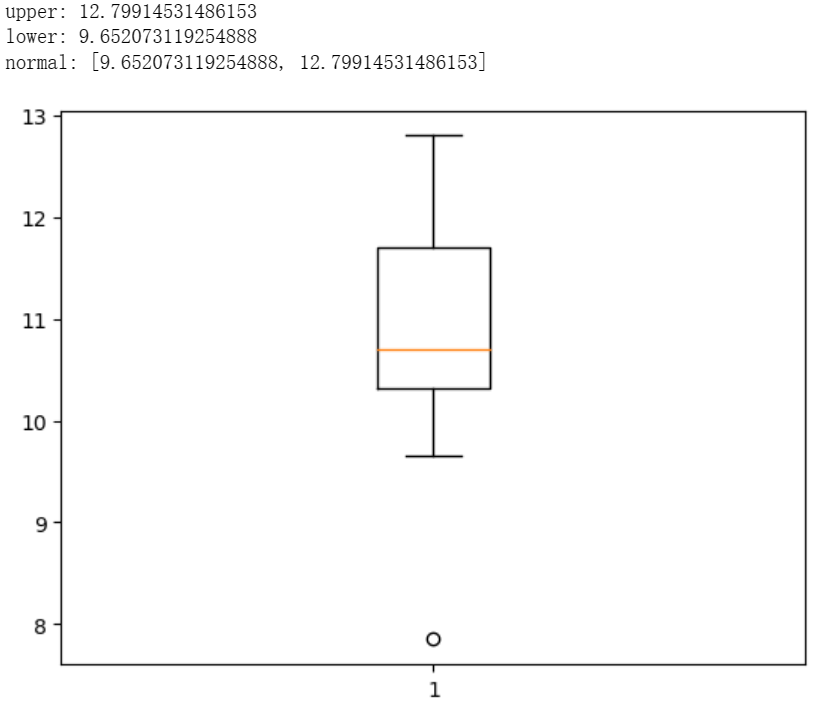
\includegraphics[width=0.5\textwidth]{3.1.4_1.png}
\caption{The box plot of the log-transformed "Number of reported results" data}
\label{fig:result}
\end{figure}


We found the data "2569" on November 30th was severely outlier, so we corrected it to "25569".

\subsubsection{Correcting the errors in the number of submissions in the hard mode}

When calculating the proportion of people choosing the hard mode on a daily basis, we found large deviations on November 1st 2022 and February 13th 2022 according to the bar graph of the hard mode ratio per week. Therefore, we revised it based on the raw report from Twitter user WordleStats.

\vspace{-0.5cm}
\begin{figure}[h!]
\centering
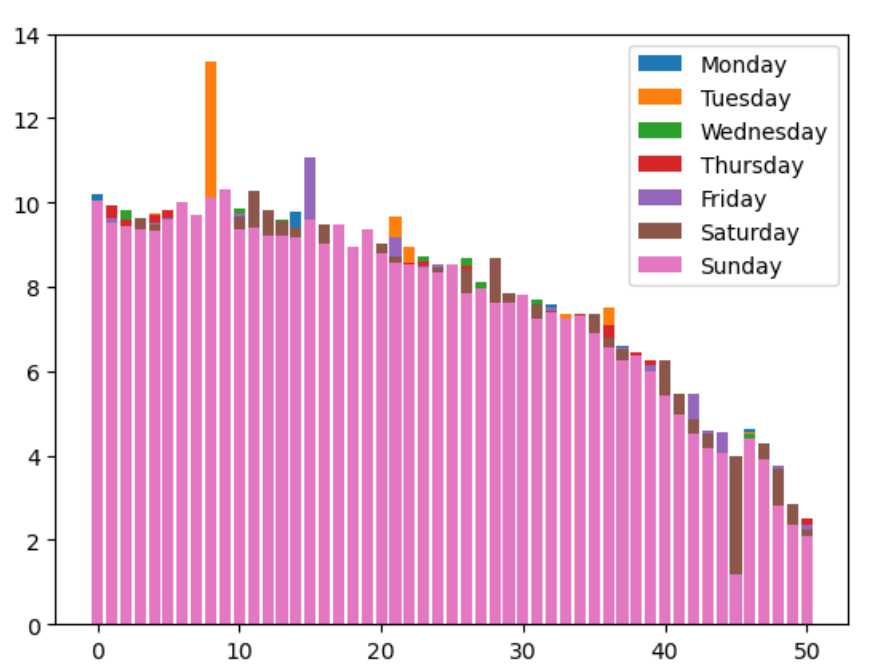
\includegraphics[width=0.5\textwidth]{3.1.5_1.png}
\caption{Bar chart of the hard mode ratio per week of seven days}
\label{fig:result}
\end{figure}

We revised the data of "3667" on November 1st to "2677" and the data of "3249" on February 13th to "9249".

\subsection{Fitting and predicting the Number of Reported Results with days}
We plotted and fitted the processed data, trying to find its patterns. After trying six models, namely polynomial, exponential, power function, rational fraction, Gaussian model and Fourier series, we found 3 fitting curves ($R^{2}$ \textgreater $\ 0.98$)  that fit the actual situation better.

\subsubsection{Polynomial Fitting}

\begin{figure}[h!]
\centering
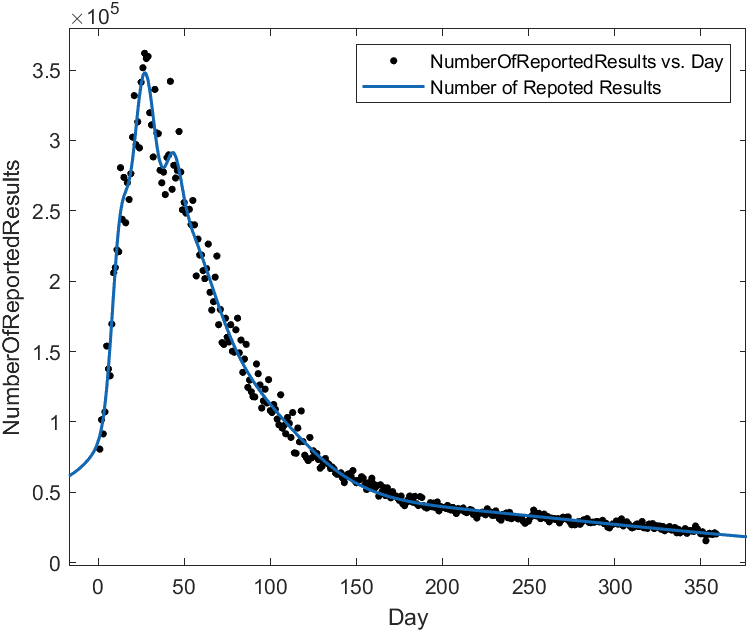
\includegraphics[width=0.6\textwidth]{3.2.1_1.png}
\caption{The result of polynomial fitting}\label{fig:result}
\end{figure}

The graph above is the result of polynomial fitting, showing the relationship between $NoRR$ and $day$:

\begin{equation}
y_1 = \sum\limits_{i=0}^9  a_ix^i
\end{equation}

With the coefficient:

\begin{table}[h]
    \caption{The coefficient of $y_1$}
    \vspace{-0.3cm}
    \begin{center}
    \begin{tabular}{| >{\centering\arraybackslash}X 
  | >{\centering\arraybackslash}X
  | >{\centering\arraybackslash}X
  | >{\centering\arraybackslash}X
  | >{\centering\arraybackslash}X
  | >{\centering\arraybackslash}X 
  | } 
    \hline
    $i$ & 0 & 1 & 2 & 3 & 4  \\ 
    \hline
    $a_i$ & $2.35 \times 10^{4}$ & $2.68 \times 10^{4}$ & $-870.1$ & $12.73$ & $-0.1069$      \\ 
    \hline
    $i$ & 5 & 6 & 7 & 8 & 9  \\ 
    \hline
    $a_i$ & $5.553 \times 10^{-4}$ & $-1.814 \times 10^{-6}$ & $3.631 \times 10^{-9}$ & $-4.063 \times 10^{-12}$ & $1.946 \times 10^{-15}$   \\
    \hline
    \end{tabular}
    \end{center}
    \label{tab:my_label}
    \vspace{-1cm}
\end{table}

\vspace{1cm}

Substituting $day=419$, we get $NoRR=2.873 \times 10^{6}$, which obviously goes against common sense.

Our analysis is that using high-order polynomial fitting can only make predictions in the region close to the known interval, because high-order terms will become very uncontrollable when the independent variable values are far away from the known interval, resulting in a large deviation of the result.


\subsubsection{Gaussian Fitting}

\begin{figure}[h!]
\centering
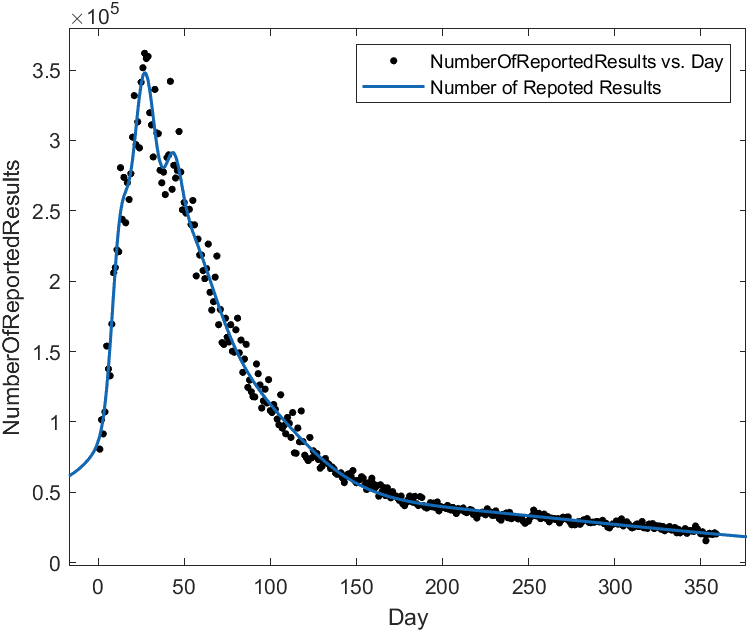
\includegraphics[width=0.6\textwidth]{3.2.2_1.png}
\caption{The result of Gaussian fitting}\label{fig:result}
\end{figure}

The graph above is the result of Gaussian fitting , showing the relationship between $NoRR$ and $day$.

\begin{equation}
y_2= \sum\limits_{i=1}^6 a_ie^{- (\frac{x-b_i}{c_i})^2 }
\end{equation}

With the coefficient:

\begin{table}[h]
    \caption{The coefficient of $y_2$}
    \vspace{-0.3cm}
    \begin{center}
    \begin{tabular}{| >{\centering\arraybackslash}X 
  | >{\centering\arraybackslash}X
  | >{\centering\arraybackslash}X
  | >{\centering\arraybackslash}X
  | >{\centering\arraybackslash}X
  | >{\centering\arraybackslash}X 
  | >{\centering\arraybackslash}X
  | } 
    \hline
    $i$ & 1 & 2 & 3 & 4 & 5 & 6  \\ 
    \hline
    $a_i/\times 10^4$ & 16.18 & 44.72 & 10.83 & 12 & 8.556 & 4.999   \\ 
    \hline
    $b_i$ & 26.08 & 43.64 & 12.64 & 43.75 & 67.06 & 28.65  \\ 
    \hline
    $c_i$ & 8.988 & 6.399 & 6.642 & 27.43 & 59.32 & 347.5   \\
    \hline
    \end{tabular}
    \end{center}
    \label{tab:my_label}
    \vspace{-1cm}
\end{table}

\vspace{1cm}

Substituting $day=419$, we get $NoRR=14154$, which is quite convincing.


\subsubsection{Fractional Fitting}

\begin{figure}[h!]
\centering
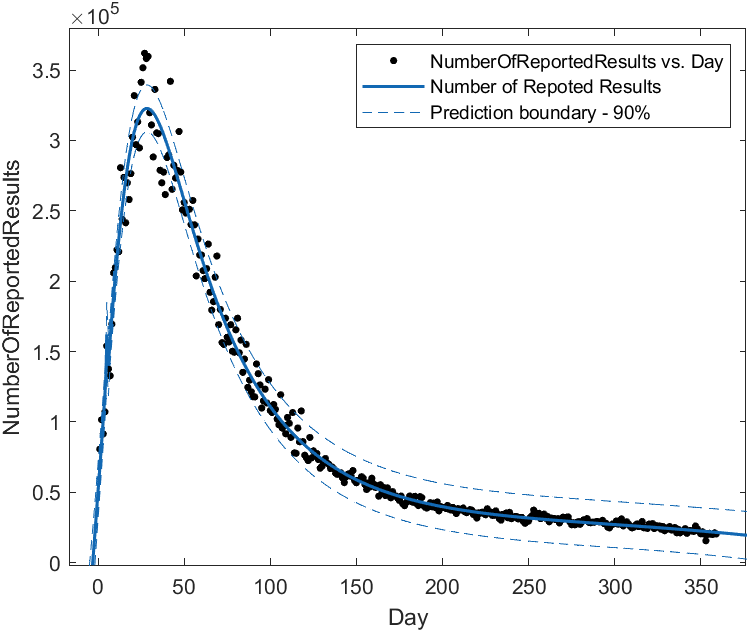
\includegraphics[width=0.6\textwidth]{3.2.3_1.png}
\caption{The result of fractional fitting}\label{fig:result}
\end{figure}

The graph above is the result of fractional fitting  , showing the relationship between $NoRR$ and $day$.
\vspace{-0.3cm}
\begin{equation}
y_3 = \frac{ \sum\limits_{i=0}^5 a_ix^i}{ \sum\limits_{j=0}^3 b_jx^j}
\end{equation}
\vspace{-0.3cm}
 
With the coefficient:
\vspace{-0.3cm}
\begin{table}[h]
    \caption{The coefficient of $y_3$}
    \vspace{-0.3cm}
    \begin{center}
    \begin{tabular}{| >{\centering\arraybackslash}X 
  | >{\centering\arraybackslash}X
  | >{\centering\arraybackslash}X
  | >{\centering\arraybackslash}X
  | >{\centering\arraybackslash}X
  | >{\centering\arraybackslash}X 
  | >{\centering\arraybackslash}X
  | } 
    \hline
    $i$ & 0 & 1 & 2 & 3 & 4 & 5  \\ 
    \hline
    $a_i$ & $-3.562 \times 10^8$ & $-4.296 \times 10^7$ & $2.212 \times 10^7$ & $-1.72 \times 10^5$ & 663.1 & -0.8292   \\ 
    \hline
    $j$ & 0 & 1 & 2 & 3 &  &  \\ 
    \hline
    $b_j$ & -6968 & 1425 & -21 & 1 &  &    \\
    \hline
    \end{tabular}
    \end{center}
    \label{tab:my_label}
    \vspace{-1cm}
\end{table}


Substituting $day=419$, we get $NoRR=13368$, which is quite convincing.

\vspace{-0.4cm}
\subsubsection{Summary}

The following are 3 types of fitting error data:

\begin{table}[h]
    \caption{Error of fitting}
    \vspace{-0.3cm}
    \begin{center}
    \begin{tabular}{| >{\centering\arraybackslash}X 
  | >{\centering\arraybackslash}X 
  | >{\centering\arraybackslash}X
  | >{\centering\arraybackslash}X
  | } 
    \hline
       & Sum of Squares for Error (SSE) & $R^2$ & Root Mean Square Error (RMSE)
  \\ 
    \hline
    Polynomial fitting & $3.87 \times 10^{10}$ & 0.9864 & $1.054 \times 10^{4}$  \\ 
    \hline
    Gaussian fitting & $2.635 \times 10^{10}$ & 0.9908 & 8790 \\ 
    \hline
    Fractional fitting & $3.427 \times 10^{10}$ & 0.988 & 9895  \\ 
    \hline
    \end{tabular}
    \end{center}
    \label{tab:my_label}
    \vspace{-0.7cm}
\end{table}

By integrating the above models, we obtain two predicted values as a prediction interval. $\widetilde{NoRR} =[13368, 14154]$



\subsection{Analysis of Association between Word Attributes and Hard Mode Rate}

Initially, we considered word attributes including the number of syllables, the number of vowel letters, the number of repeated letters, and word frequency, and divided the given words according to their attributes.
\vspace{-0.7cm}
\subsubsection{Number of Syllables}
\vspace{-0.8cm}
%组图
            \begin{figure*}[h]
                \centering
                \begin{subfigure}[b]{0.4\textwidth}
                    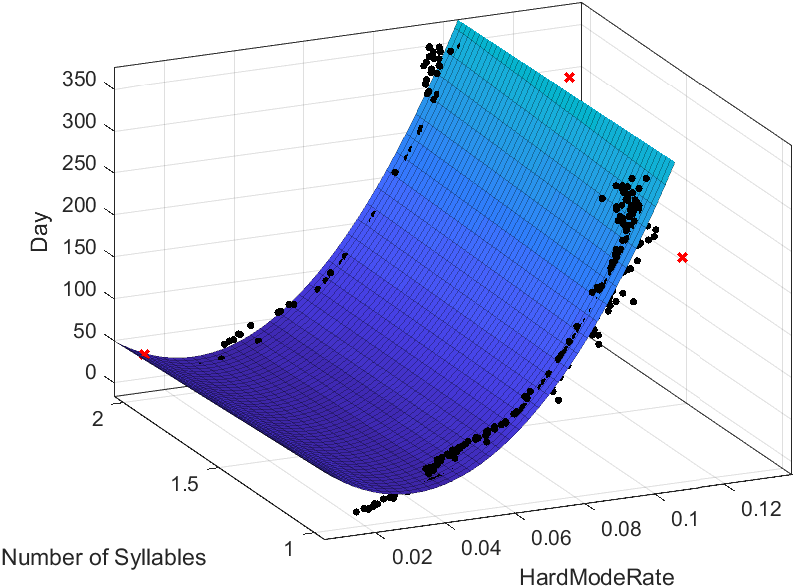
\includegraphics[width=\textwidth]{3.3.1_1.png}
                    \caption{3D fitting}
                \end{subfigure}
                \begin{subfigure}[b]{0.4\textwidth}
                    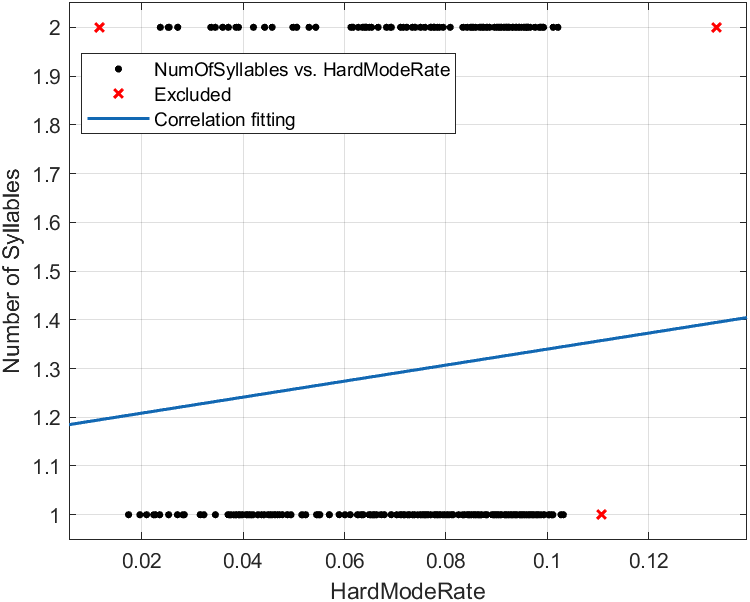
\includegraphics[width=\textwidth]{3.3.1_2.png}
                    \caption{2D fitting}
                \end{subfigure}
                \caption{the correlation coefficient between Hard Mode Rate and Number of Syllables}
            \end{figure*}

Then, we plotted the graph and calculated the correlation coefficient between the Hard Mode Rate and the Number of Syllables $R^{2}=5.989 \times   10^{-3}$, so it can be concluded that the Number of Syllables is not correlated with Hard Mode Rate.
\vspace{-0.7cm}
\subsubsection{Number of Vowels}

%组图
            \begin{figure*}[h]
                \centering
                \begin{subfigure}[b]{0.4\textwidth}
                    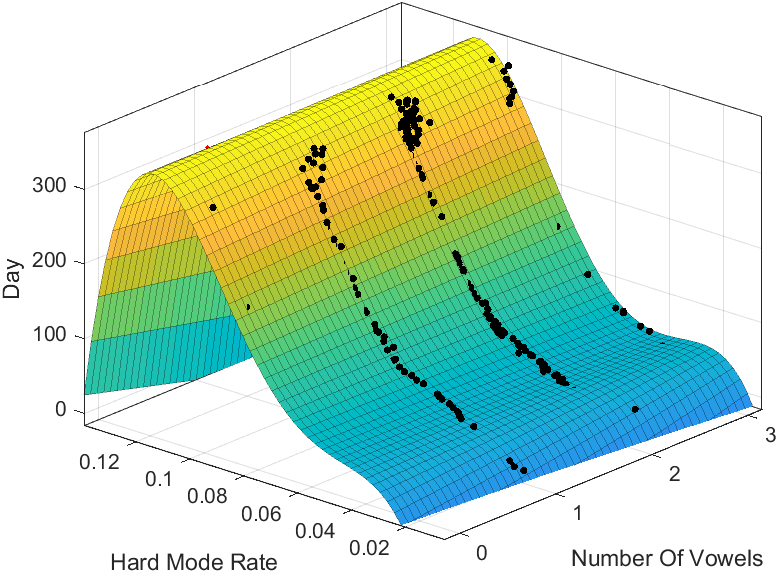
\includegraphics[width=\textwidth]{3.3.2_1.png}
                    \caption{3D fitting}
                \end{subfigure}
                \begin{subfigure}[b]{0.4\textwidth}
                    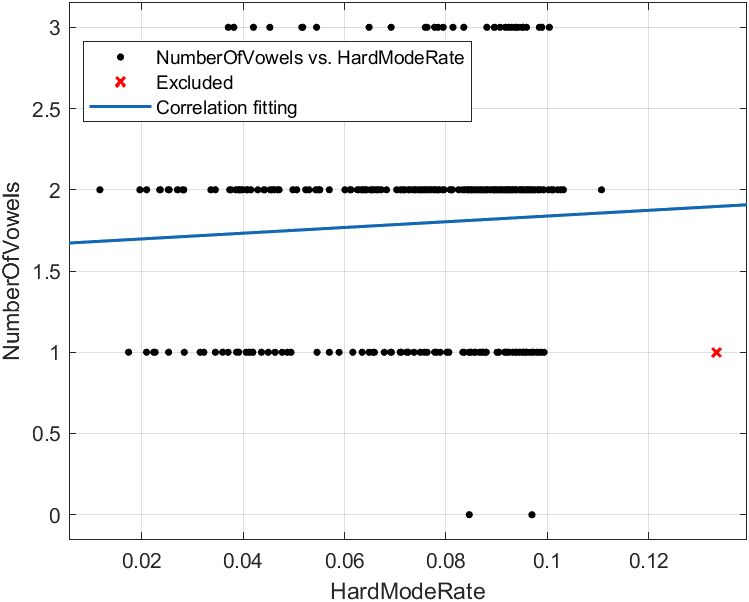
\includegraphics[width=\textwidth]{3.3.2_2.png}
                    \caption{2D fitting}
                \end{subfigure}
                \caption{the squared correlation coefficient between Hard Mode Rate and Number of Vowels}
            \end{figure*}

We plotted the graph and calculated the squared correlation coefficient $R^{2}=4.086 \times   10^{-3}$ between the Hard Mode Rate and the Number of Vowels, so it can be concluded that the Number of Vowels is not correlated with the Hard Mode Rate.


\subsubsection{Number of Repeated Letters}

%组图
            \begin{figure*}[h]
                \centering
                \begin{subfigure}[b]{0.4\textwidth}
                    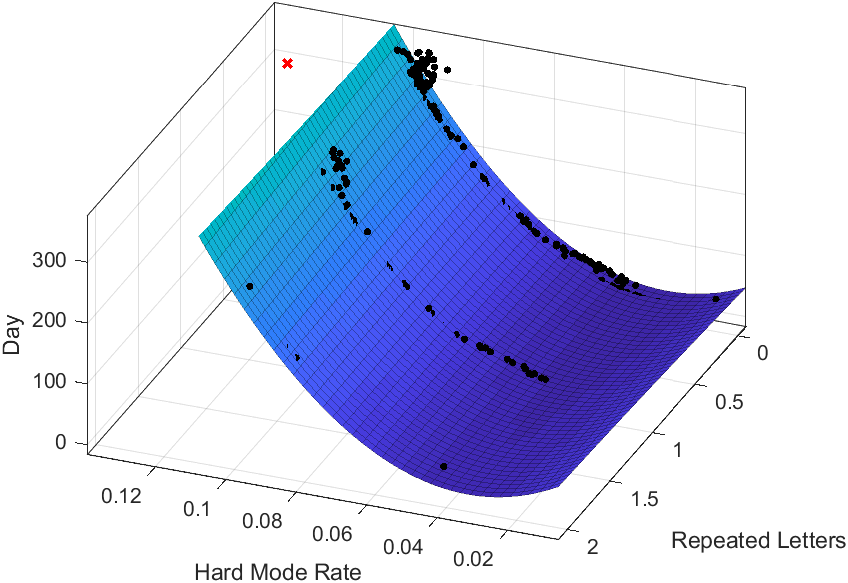
\includegraphics[width=\textwidth]{3.3.3_1.png}
                    \caption{3D fitting}
                \end{subfigure}
                \begin{subfigure}[b]{0.4\textwidth}
                    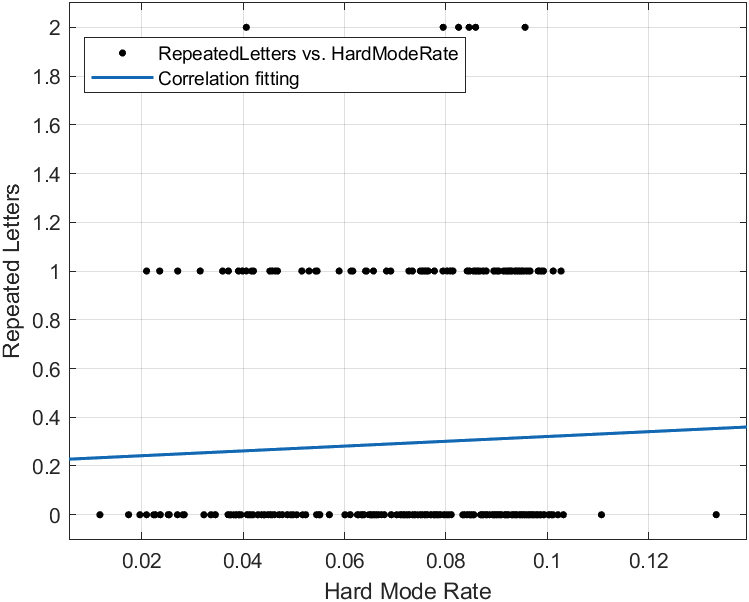
\includegraphics[width=\textwidth]{3.3.3_2.png}
                    \caption{2D fitting}
                \end{subfigure}
                \caption{the squared correlation coefficient between Hard Mode Rate and Number of Repeated Letters}
            \end{figure*}

We plotted the graph and calculated the squared correlation coefficient $R^{2}=1.951 \times   10^{-3}$ between the Hard Mode Rate and the Number of Repeated Letters, so it can be concluded that the Number of Repeated Letters is not correlated with the Hard Mode Rate.

\subsubsection{Word Frequency}


            \begin{figure*}[h]
                \centering
                \begin{subfigure}[b]{0.4\textwidth}
                    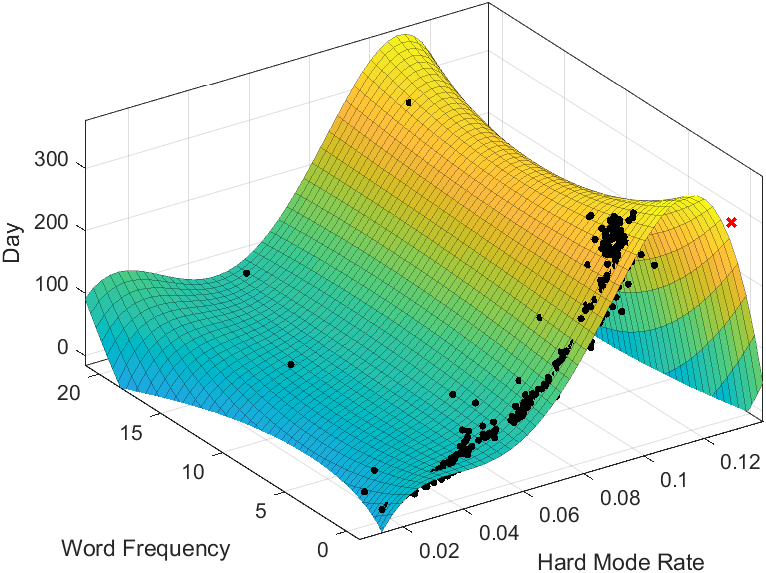
\includegraphics[width=\textwidth]{3.3.4_1.png}
                    \caption{3D fitting}
                \end{subfigure}
                \begin{subfigure}[b]{0.4\textwidth}
                    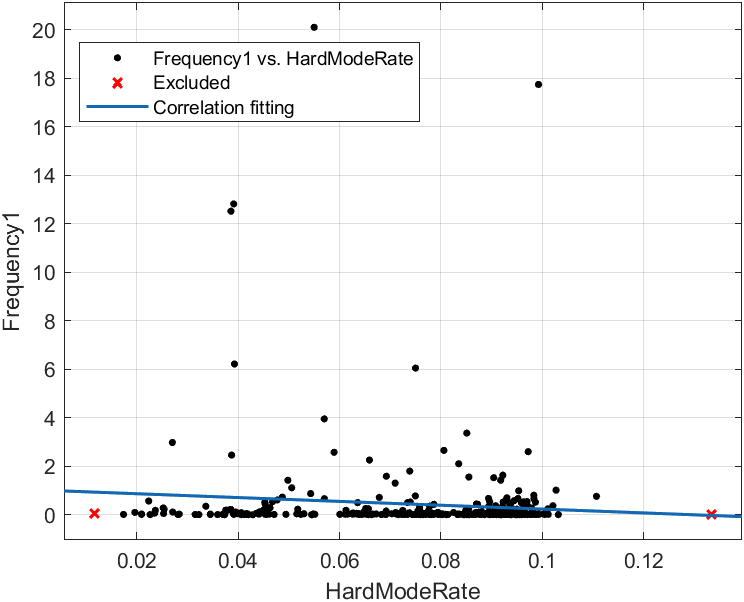
\includegraphics[width=\textwidth]{3.3.4_2.png}
                    \caption{2D fitting}
                \end{subfigure}
                \caption{the squared correlation coefficient between Hard Mode Rate and Word Frequency}
            \end{figure*}

We plotted the graph and calculated the squared correlation coefficient between the Hard Mode Rate and the Word Frequency  $R^{2}=8.968 \times   10^{-3}$, so it can be concluded that the Word Frequency is not correlated with the Hard Mode Rate.

\subsubsection{Summary}
We considered the four word attributes including the number of syllables, the number of vowel letters, word frequency, and the number of repeated letters, and fitted data to find their linear correlation coefficients all in an order of magnitude $10^{-2}$, which is much lower than statistically $R\  \geq \ 0.75$ considered to be related between two groups of data, we can conclude that the word attributes we have considered are not correlated with the proportion of selecting Hard Mode Rate.


\subsection{Classification of Word Difficulty}

\subsubsection{Constructing Evaluation Criteria for Word Difficulty}

We conducted statistics and following is the table that shows the average percentage of tries.

\begin{table}[h]
    \caption{Tries average percentage}
    \vspace{-0.3cm}
    \begin{center}
    \begin{tabular}{| >{\centering\arraybackslash}X 
  | >{\centering\arraybackslash}X 
  | >{\centering\arraybackslash}X
  | >{\centering\arraybackslash}X
  | >{\centering\arraybackslash}X
  | >{\centering\arraybackslash}X
  | >{\centering\arraybackslash}X
  | >{\centering\arraybackslash}X
  | } 
    \hline
    Tries/$i$ & 1 & 2 & 3 & 4 & 5 & 6 & X
  \\ 
    \hline
    Percentage/\% & 0.5 & 6.0 & 22.5 & 33.0 & 23.5 & 11.5 & 3.0
      \\ 
    \hline
    \end{tabular}
    \end{center}
    \label{tab:my_label}
    \vspace{-0.7cm}
\end{table}

Due to Wordle being a global daily question, its answers are easily spread through the internet, making it easy for users to get the answers directly;  since Wordle is an open-source project written in JavaScript, its source code is also open, so it can be viewed directly to get all the answers; furthermore, the possibility of guessing the correct answer after only one or two attempts is very small, but the chance of it being a coincidence is high. Therefore, we did not include data with only 1 or 2 tries in the difficulty rating.


We assign a difficulty score to attempts from 3 to 6 and X respectively, with higher scores indicating easier difficulty. We believe that the difficulty score is inversely proportional to the number of attempts, i.e. the higher the difficulty, the more attempts are required inversely. We also assume that probability is proportional to difficulty score, i.e. the easier it is for this attempt to occur, the higher the difficulty score will be as players are more likely to achieve this situation.

so we can get: $s_i=\begin{cases} 
 \frac{ \overline{p_i} }{i}  & i = 3,4,5,6 \\ 0 & i = 1,2,X
\end{cases} $

\begin{table}[h]
    \caption{Tries difficulty score}
    \vspace{-0.3cm}
    \begin{center}
    \begin{tabular}{| >{\centering\arraybackslash}X 
  | >{\centering\arraybackslash}X 
  | >{\centering\arraybackslash}X
  | >{\centering\arraybackslash}X
  | >{\centering\arraybackslash}X
  | >{\centering\arraybackslash}X
  | >{\centering\arraybackslash}X
  | >{\centering\arraybackslash}X
  | } 
    \hline
    Tries/$i$ & 1 & 2 & 3 & 4 & 5 & 6 & X
  \\ 
    \hline
    
    \toprule [1pt]
    $s_{t\_i}$ & 0 & 0 & $\frac{22.5}{3}  =7.50$ & $\frac{33}{4}  =8.25$ & $\frac{23.5}{5}  =4.70$ & $\frac{11.5}{6} \approx 1.92$ & 0
      \\ 
    \hline
    \end{tabular}
    \end{center}
    \label{tab:my_label}
    \vspace{-0.7cm}
\end{table}

Then we can calculate the difficulty score corresponding to each day's words:
\begin{equation}
s_{day=t}= \sum\limits_{i=3}^6 p_{t\_i}s_i
\end{equation}

After calculating the difficulty score for all words,we calculate the correlation coefficient squared (here referred to as $R_1^2$, $R_2^2$, $R_3^2$, $R_4^2$) for each of the four-word attributes considered.

\begin{table}[h]
    \caption{Correlation coefficient squared}
    \vspace{-0.3cm}
    \begin{center}
    \begin{tabular}{| >{\centering\arraybackslash}X 
  | >{\centering\arraybackslash}X 
  | >{\centering\arraybackslash}X
  | >{\centering\arraybackslash}X
  | >{\centering\arraybackslash}X
  | >{\centering\arraybackslash}X
  | } 
    \hline
     & Syllables & Vowels & Repeated Letters & Frequency \\ 
    \hline
    $s$ & 0.0007834 & 0.0023893 & 0.0486970 & 0.0007240  \\ 
    \hline
    \end{tabular}
    \end{center}
    \label{tab:my_label}
    \vspace{-0.7cm}
\end{table}

We found that ${R_3} ^{2} \gg{R_2} ^{2} \gg{R_1} ^{2} \approx{R_4} ^{2}$ , so the main influencing factors for word difficulty could be determined to be the number of repeated letters and the number of vowels. To give each data point a certain distinction, we classified the data points while adding a word attribute of frequency (but not as a main classification criterion).


The K-means Clustering Algorithm is a iterative clustering analysis algorithm which steps are to pre-divide the data into K groups, then randomly select K objects as initial cluster centers, calculate the distance between each object and each seed cluster center, and assign each object to the closest cluster center. The clusters centers and the objects assigned to them represent a cluster. Every time a sample is assigned, the clusters' cluster centers will be re-calculated according to the existing objects in the clusters. This process will keep repeating until some termination condition is met.

Using clustering analysis based on the K-means algorithm (Matlab code in Appendix), we divided words into four categories: Less Vowels Less Repeated Letters, Less Vowels More Repeated Letters, More Vowels Less Repeated Letters, More Vowels More Repeated Letters. The classification results are shown in the figure below:

\vspace{0.7cm}
\begin{figure*}[h]
    \centering
        \begin{subfigure}[b]{0.4\textwidth}
            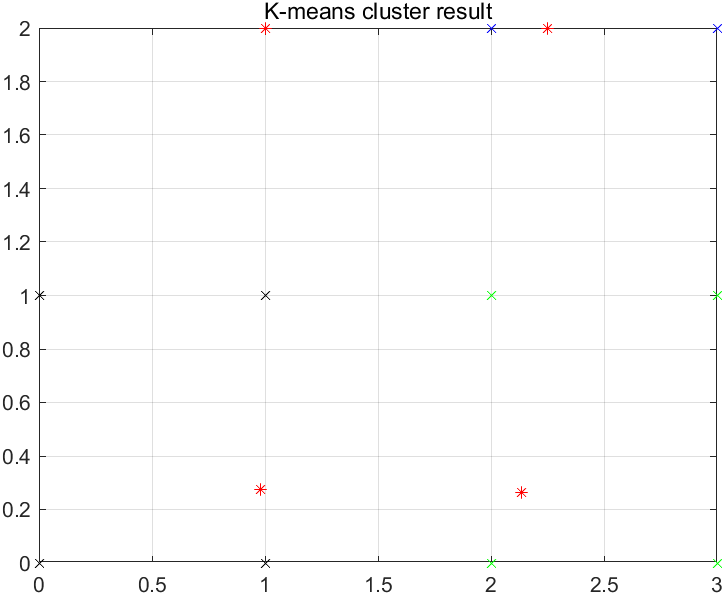
\includegraphics[width=\textwidth]{3.4.1_1.png}
            \caption{Result without coordinate}
        \end{subfigure}
        \begin{subfigure}[b]{0.4\textwidth}
            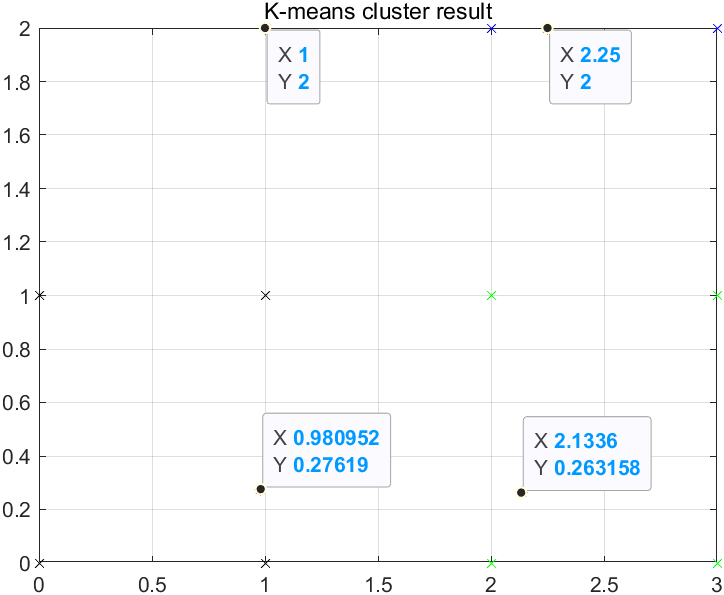
\includegraphics[width=\textwidth]{3.4.1_2.png}
            \caption{Result with coordinate}
        \end{subfigure}
        \caption{2D K-means cluster result}
\end{figure*}

The X and Y axes in the graph represent the number of vowels and the number of repeated letters respectively. The black, yellow, green, and blue x-shaped points represent data points from the first to fourth categories respectively, while the red point represents the center point of each category with coordinates as shown in the right graph.

As only the number of vowels and repeated letters were taken into consideration, there was a high degree of overlap between data points and insufficient distinction. In order to increase data distinction and enhance intuitiveness,we also take frequency   into consideration as a word attribute for reclassification and plotting. The result is in the following graph. Where Z axis is word frequency($\times  10^{4}$).

\begin{figure*}[h]
    \centering
        \begin{subfigure}[b]{0.4\textwidth}
            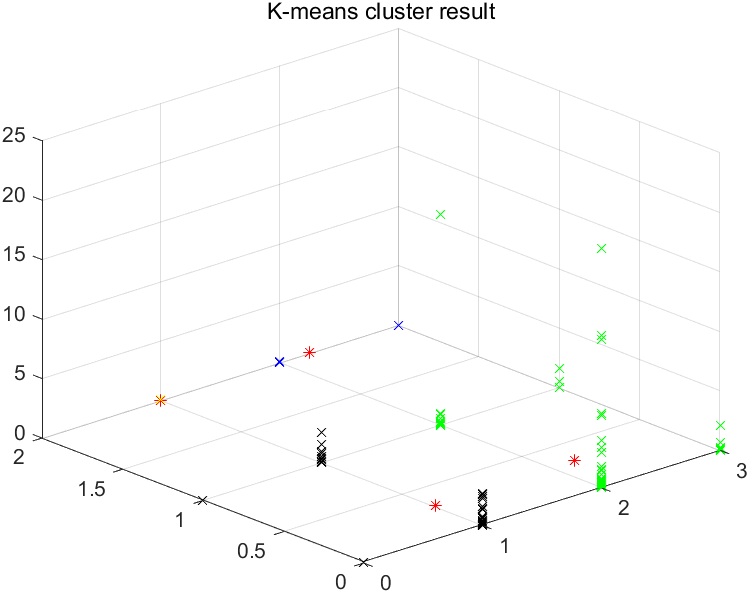
\includegraphics[width=\textwidth]{3.4.1_3.png}
            \caption{Result without coordinate}
        \end{subfigure}
        \begin{subfigure}[b]{0.4\textwidth}
            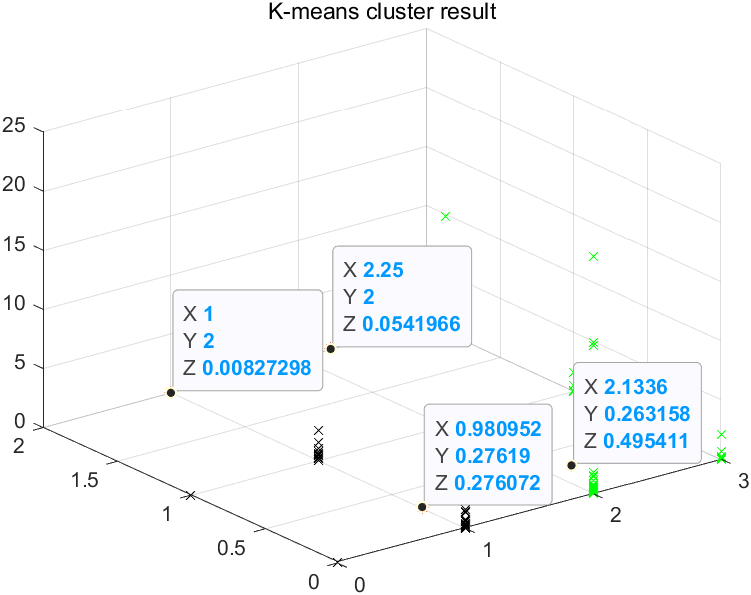
\includegraphics[width=\textwidth]{3.4.1_4.png}
            \caption{Result with coordinate}
        \end{subfigure}
        \caption{3D K-means cluster result}
        \vspace{-0.5cm}
\end{figure*}


\vspace{9cm}

\subsubsection{Analysis of the word EERIE}
The word EERIE has three vowels and two repeated letters, and the Euclidean distance from the center of Class 4 (blue data points) is closest, so it is classified as Class 4 according to the figure.

The table below shows the words in Class 4 and their corresponding difficulty scores:
\vspace{-0.4cm}
\begin{table}[h]
    \caption{Difficulty score for errie}
    \vspace{-0.5cm}
    \begin{center}
    \begin{tabular}{| >{\centering\arraybackslash}X 
  | >{\centering\arraybackslash}X 
  | >{\centering\arraybackslash}X 
  | >{\centering\arraybackslash}X 
  | >{\centering\arraybackslash}X 
  | >{\centering\arraybackslash}X 
  | } 
    \hline
      & vivid & cacao & madam & motto & AVG \\ [0.5ex] 
    \hline
    difficulty score & 509.67 & 503.61 & 572.93 & 575.58 & 540.45 \\ 
    \hline
    \end{tabular}
    \end{center}
    \label{tab:my_label}
\end{table}
\vspace{-1cm}

Taking the average of 540.45 as the difficulty score for EERIE, we found that it ranked 77th out of 360 words, which is approximately 20\% of the total words. This indicates that EERIE is a relatively difficult word.

The 10 words with the closest difficulty to EERIE (from hardest to easiest) are: 
\vspace{-0.5cm}
\begin{table}[h]
    \caption{Words closest to EERIE}
    \vspace{-0.5cm}
    \begin{center}
    \begin{tabular}{| >{\centering\arraybackslash}X 
  | >{\centering\arraybackslash}X 
  | >{\centering\arraybackslash}X 
  | >{\centering\arraybackslash}X 
  | >{\centering\arraybackslash}X 
  | >{\centering\arraybackslash}X 
  | >{\centering\arraybackslash}X 
  | >{\centering\arraybackslash}X 
  | >{\centering\arraybackslash}X 
  | >{\centering\arraybackslash}X 
  | } 
    \hline
     stead& movie& grate& shall& shard& slate& query& epoxy& foray& stair\\
    \hline
    \end{tabular}
    \end{center}
    \label{tab:my_label}
\end{table}
\vspace{-1cm}

\subsection{Prediction of the distribution of relevant percentages (1, 2, 3, 4, 5, 6, X)}
The following table shows the percentage of attempts for category 4 data points:

\begin{table}[h]
    \caption{difficulty score}
    \vspace{-0.5cm}
    \begin{center}
    \begin{tabular}{| >{\centering\arraybackslash}X 
  | >{\centering\arraybackslash}X 
  | >{\centering\arraybackslash}X 
  | >{\centering\arraybackslash}X 
  | >{\centering\arraybackslash}X 
  | >{\centering\arraybackslash}X 
  | >{\centering\arraybackslash}X 
  | >{\centering\arraybackslash}X 
  | } 
    \hline
    Word & 1 try & 2 tries & 3 tries & 4 tries & 5 tries & 6 tries & X \\ [0.5ex] 
    \hline
    vivid & 1 & 2 & 10 & 29 & 33 & 21 & 4 \\ 
    \hline
    cacao & 0 & 1 & 9 & 27 & 36 & 23 & 4 \\ 
    \hline
    madam & 0 & 3 & 13 & 35 & 34 & 14 & 2 \\ 
    \hline
    motto & 0 & 1 & 11 & 36 & 36 & 14 & 1 \\ 
    \hline
    AVG & 0 & 2 & 11 & 32 & 35 & 18 & 3 \\ 
    \hline
    SrDev & 0.50 & 0.96 & 1.71 & 4.43 & 1.50 & 4.60 & 1.50 \\ 
    \hline
    \end{tabular}
    \end{center}
    \label{tab:my_label}
    
    \end{table}
We calculated the mean (rounded) and standard deviation of each attempt, and  found that the standard deviation was within an acceptable range, so we chose the mean as the predicted value for the word EERIE.

The following table  shows the predicted values for EERIE:

\begin{table}[h]
    \caption{difficulty score}
    \vspace{-0.5cm}
    \begin{center}
    \begin{tabular}{| >{\centering\arraybackslash}X 
  | >{\centering\arraybackslash}X 
  | >{\centering\arraybackslash}X 
  | >{\centering\arraybackslash}X 
  | >{\centering\arraybackslash}X 
  | >{\centering\arraybackslash}X 
  | >{\centering\arraybackslash}X 
  | >{\centering\arraybackslash}X 
  | } 
    \hline
    Word & 1 try & 2 tries & 3 tries & 4 tries & 5 tries & 6 tries & X \\ [0.5ex] 
    \hline
    eerie & 0 & 2 & 11 & 32 & 35 & 18 & 3 \\  
    \hline
    \end{tabular}
    \end{center}
    \label{tab:my_label}

\end{table}



\subsection{ Other characteristics of the data set}
\subsubsection{The impact of holidays on the reported results}
In order to explore the impact of holidays on the number of players, we labeled each day of the week and counted the number of submissions in the given data for 51 weeks, creating a histogram.

\begin{figure}[h!]
\centering
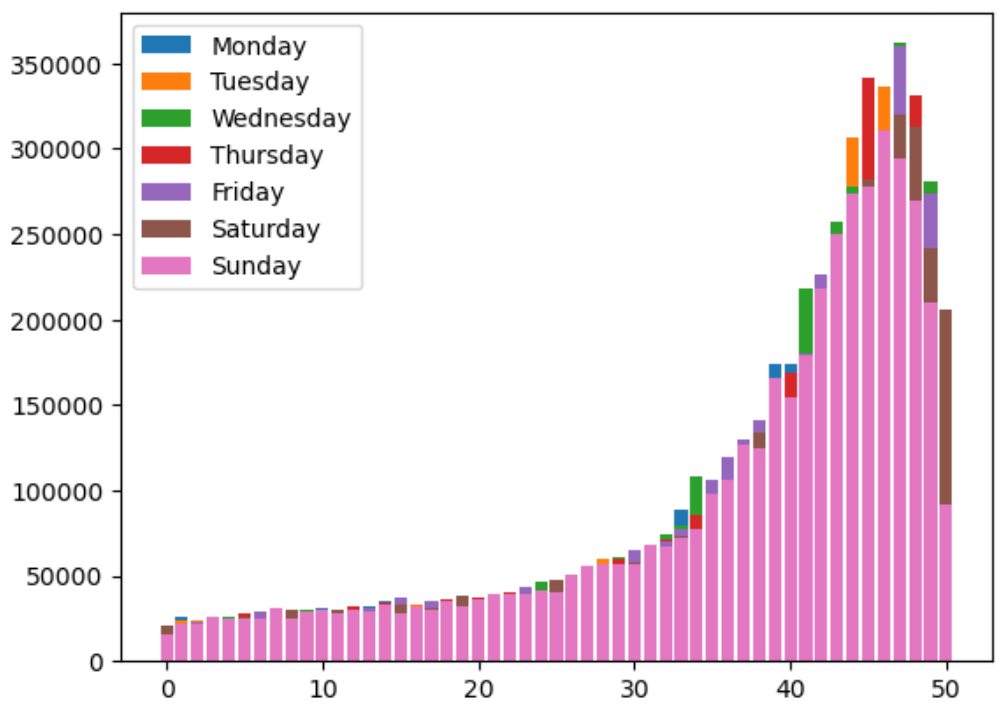
\includegraphics[width=0.7\textwidth]{3.6.1_1.png}
\caption{Histogram of 51-week submitter by one-week label}\label{fig:result}
\end{figure}

From the above graph, it is clear that Sunday is represented by the pink color, which is the lowest in terms of the number of submissions. This indicates that Sunday has the least number of game submissions. Thus, we can infer that Wordle is a game more suited for filling up short periods of time, and when weekends arrive people tend to opt for more wholesome forms of leisure instead of Wordle.

\subsubsection{The impact of the proportion of people who choose Hardmode }
In order to explore the relationship between the percentage of players selecting the difficult mode and time, we labeled each day of the week and counted the percentage of players selecting the difficult mode in the given data for 51 weeks, creating a histogram.

\begin{figure}[h!]
\centering
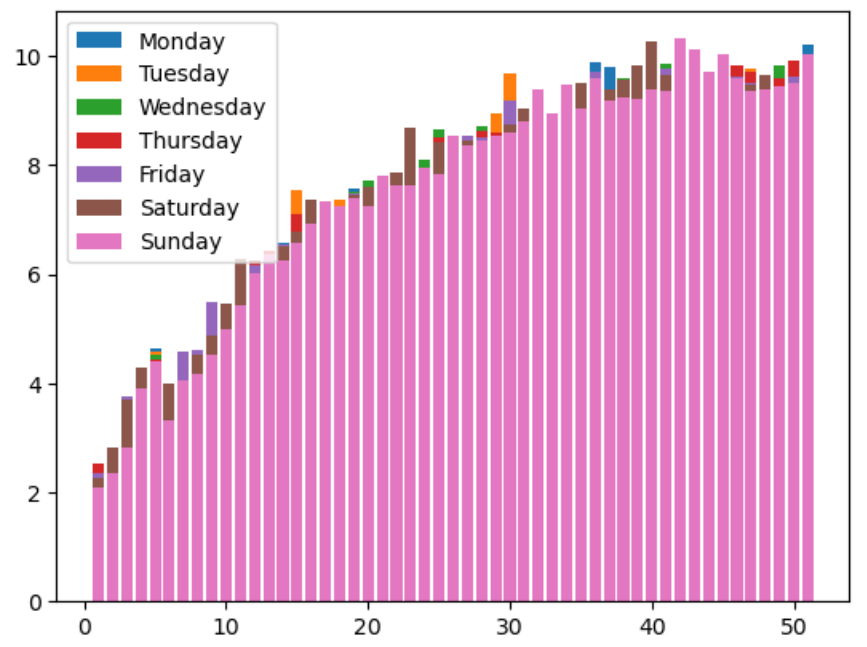
\includegraphics[width=0.7\textwidth]{3.6.2_1.png}
\caption{Percentage histogram with Hard mode selected}\label{fig:result}
\end{figure}

 As time progresses, the percentage of players selecting the difficult mode increases and eventually converges to an average value. This suggests that as people become more familiar with the game, their willingness to take on a challenging difficulty level also increases.


\subsubsection{The impact of lexical category }

From the analysis of the British National Corpus (BNC) with 8,000 frequently used words merged with Daily Words, 106 words, and 127-word types were obtained and ranked.

\vspace{-0.5cm}
\begin{table}[h]
    \caption{The correspondence between part of speech and frequency}
    \vspace{-0.5cm}
    \begin{center}
    \begin{tabular}{| >{\centering\arraybackslash}X 
  | >{\centering\arraybackslash}X 
  | >{\centering\arraybackslash}X 
  | >{\centering\arraybackslash}X 
  | >{\centering\arraybackslash}X 
  | >{\centering\arraybackslash}X 
  | >{\centering\arraybackslash}X 
  | >{\centering\arraybackslash}X 
  | >{\centering\arraybackslash}X 
  | } 
    \hline
    NoC & Verb & Adj & Adv & DetP & VMod & Ord & Ex & Det\\ [0.5ex] 
    \hline
    64 & 30 & 21 & 5 & 2 & 2 & 1 & 1 & 1 \\ 
    \hline
    \end{tabular}
    \end{center}
    \label{tab:my_label}
    \vspace{-1cm}
\end{table}

 We found that nouns, verbs, and adjectives are the most frequent in questions, and 21 words have two-word types accounting for 19.8\%. It can be inferred that question makers are more inclined to nouns and words with multiple word types.


\section{Strengths and Weaknesses}
\subsection{Strengths}
\subsubsection{Benefits of function fitting}
\begin{itemize}
    \item Polynomial function fitting modeling is fast and it is effective for small data sets.
    \item The model is easy to understand, which helps in decision analysis.
\end{itemize}
\subsubsection{Advantages of clustering}
\begin{itemize}
    \item The algorithm is simple and clear.
    \item It can use the information of multiple variables to classify the samples.
    \item The classification results are intuitive and the cluster phylogenetic tree clearly shows its numerical classification results. 
    \item The results obtained from clustering analysis are more detailed, comprehensive, and reasonable than traditional classification methods.
\end{itemize}

\subsection{Weaknesses}
\subsubsection{Disadvantages of function fitting}
\begin{itemize}
    \item For nonlinear data or difficult modeling, it is difficult to express highly complex data well.
 \end{itemize}
\subsubsection{Disadvantages of clustering methods}
\begin{itemize}
    \item The algorithm has a high time complexity.
    \item The process is irreversible.
    \item The clustering termination conditions are imprecise.
    \item The effect is not good when the data size is small.

\end{itemize}


% 以下为信件/备忘录部分,不需要可自行去掉
% 如有需要可将整个 letter 环境移动到文章开头或中间
% 请在第二个花括号内填写标题,如「信件」(Letter)或「备忘录」(Memorandum)
\begin{letter}{Letter}
\begin{flushleft}  % 左对齐环境,无首行缩进
\textbf{To:} The Puzzle Editor of the New York Times\\
\textbf{From:} Team 2318758\\
\textbf{Date:} February 20th, 2023\\
\textbf{Subject:} Analysis and Suggestions on Wordle
\end{flushleft}

Thanks for your invitation to the famous game Wordle's research. In the last 4 days, we use the information you bring to us and some information from the website and developed some models to predict and analyze. Now we are introducing our analysis of the prediction results for Wordle.
 
 Firstly, based on the statistics from Twitter, we found that the number of reported results is changing every day. Therefore, we employed a function fitting method to fit the data in 2022 and compared the fitting results. We found that Gaussian fitting and fractional fitting give more convincing predictions. The predicted interval of reported result numbers on March 1st, 2023 is between 13368 and 14154. 
 
Secondly, we achieved a prediction interval for Reported Result numbers on March 1st, 2023, and analyzed whether some attributes of words would affect the proportion of players choosing Hard Mode; We developed a model to predict Reported Result distribution (which enables us to predict given words in future date). To present our model more intuitively, we took Wordle's prediction for the word EERIE on March 1st, 2023 as an example and discussed uncertainties existing in our model and prediction.

 Meanwhile, we used cluster analysis to classify word difficulty to judge EERIE's difficulty level and discussed the accuracy of classification models. Moreover, during the data analysis process, some interesting features were also discovered such as fewer reports on Sundays; a gradually increasing proportion selecting Hard Mode which tends towards stability; answers more likely being nouns or multi-word units. 
 
Finally, after several days of research work, we find it necessary to increase play ability for Wordle can gain more users and loyalty. Here are several suggestions: 
\begin{itemize}
    \item Increasing game diversity by changing length or type of words offers users novel experiences while increasing user loyalty at same time.
    \item Adding social properties can increase themes so different kinds of users can use different themes; ranking mechanism can be adopted too with help from friends' social dissemination power making game even more popular.
\end{itemize}


According to all those mentioned above, it is really worth to have a try! 

\begin{flushright}

Sincerely, Team 2318758
\end{flushright}

\end{letter}


% 参考文献,此处以 MLA 引用格式为例



% 以下为附录内容
% 如您的论文中不需要附录,请自行删除
\begin{subappendices}  % 附录环境
\begin{thebibliography}{99}  
\bibitem{ref1}
Yuri Lin, Jean-Baptiste Michel, Erez Lieberman Aiden, Jon Orwant, William Brockman, Slav Petrov. Syntactic Annotations for the Google Books Ngram Corpus. Proceedings of the 50th Annual Meeting of the Association for Computational Linguistics Volume 2: Demo Papers (ACL '12) (2012)
\bibitem{ref2}http://www.natcorp.ox.ac.uk/using/index.xml?ID=freq

\end{thebibliography}


\clearpage

\section{Appendix: Program Codes}
Here are the program codes we used in our research.

% 代码环境示例三则
% 如您的论文不需要展示代码,请删除
% 更多用法,请参考 listings 宏包文档

\begin{lstlisting}[language=MATLAB, name={K_means.m}]
function [Idx, Center] = K_means(X, xstart)

% K-means
% Idx is the mark of which class the data point belongs to
% Center is the central location of each class
% X are all 3D data points
% xstart is the initial center position of the class

len = length(X);        
Idx = zeros(len, 1);    % The Id of each data point, which is the class

C1 = xstart(1,:);       
C2 = xstart(2,:);       
C3 = xstart(3,:);       
C4 = xstart(4,:);      

for i_for = 1:100
    
    % Which class does the update data point belong to
    for i = 1:len
        x_temp = X(i,:);    % Extract a single data point
        d1 = norm(x_temp - C1);    
        d2 = norm(x_temp - C2);    
        d3 = norm(x_temp - C3);    
        d4 = norm(x_temp - C4);    
        d = [d1;d2;d3;d4];
        [~, id] = min(d);   % The nearest class belongs to that class
        Idx(i) = id;
    end
    
    % Update the central location of the class
    L1 = X(Idx == 1,:);     
    L2 = X(Idx == 2,:);     
    L3 = X(Idx == 3,:);    
    L4 = X(Idx == 4,:);     
    C1 = mean(L1);      
    C2 = mean(L2);      
    C3 = mean(L3);      
    C4 = mean(L4);    
end

Center = [C1; C2; C3; C4];
\end{lstlisting}

\begin{lstlisting}[language=MATLAB, name={Test_K_means.m}]
%% K-means cluster
X = [x1; x2; x3; x4];  % Data points to be clustered
xstart = [0.5 0.5 0.42; 2.5 0.5 0.42; 0.5 1.5 0.42; 2.5 1.5 0.42];  
% Initial cluster center

[Idx, Center] = K_means(X, xstart);

figure;
plot3(X(Idx==1,1), X(Idx==1,2), X(Idx==1,3), 'kx'); hold on
plot3(X(Idx==2,1), X(Idx==2,2), X(Idx==2,3), 'gx');
plot3(X(Idx==3,1), X(Idx==3,2), X(Idx==3,3), 'yx');
plot3(X(Idx==4,1), X(Idx==4,2), X(Idx==4,3), 'bx');
plot3(Center(:,1), Center(:,2), Center(:,3), 'r*'); hold off
grid on;
title('K-means cluster result');

disp('xstart = ');
disp(xstart);
disp('Center = ');
disp(Center);
\end{lstlisting}

\begin{lstlisting}[language=PYTHON, name={clean.ipynb}]
wordle = pd.read_excel("Problem_C_Data_Wordle.xlsx")
def function(a, b, c, d, e, f, g):
    return a + b + c + d + e + f + g
wordle['sum'] = wordle.apply(
    lambda x: function(x[5], x[6], x[7],
    x[8], x[9], x[10], x[11]), axis=1)
ab = pd.DataFrame(wordle['sum'].value_counts())
abnormal = wordle.loc[(wordle['sum'] == 126) 
| (wordle['sum'] == 102) | (wordle['sum'] == 98), ['Date', 'sum']]
wordle.loc[279, '4 tries'] = 44
wordle.loc[279, '5 tries'] = 26
wordle.loc[279, '6 tries'] = 9
wordle.loc[279, '7 or more tries (X)'] = 1
del wordle['sum']
def word(a):
    return len(a)
wordle['len'] = wordle.apply(lambda x: word(x[2]), axis=1)
wordle['len'].value_counts()
abnormal = wordle.loc[(wordle['len'] != 5), ['Date', 'len', 'Word']]
wordle.loc[15, 'Word'] = 'probe'
wordle.loc[35, 'Word'] = 'clean'
wordle.loc[246, 'Word'] = 'trash'
wordle.loc[353, 'Word'] = 'favor'
del wordle['len']
lista=['a','b','c','d','e','f','g','h','i'
        ,'j','k','l','m','n','o','p','q','r'
        ,'s','t','u','v','w','x','y','z']
def wordc(a):
    for i in a:
        if i not in lista:
            return False
    return True  
wordle['worda'] = wordle.apply(lambda x: wordc(x[2]), axis=1)
wordle[wordle['worda'] == False]
wordle.loc[20,'Word']='naive'
bp = plt.boxplot(wordle['Number of  reported results'])
lower_whisker = [item.get_ydata()[1] for item in bp['whiskers']][0]
upper_whisker = [item.get_ydata()[1] for item in bp['whiskers']][1]
def log(a):
    return math.log(a)
wordle['Number of log reported results'] = wordle.apply(
    lambda x: log(x['Number of  reported results']), axis=1)
bp = plt.boxplot(wordle['Number of log reported results'])
lower_whisker = [item.get_ydata()[1] for item in bp['whiskers']][0]
upper_whisker = [item.get_ydata()[1] for item in bp['whiskers']][1]
ob = wordle[(wordle['Number of log reported results'] < lower_whisker) |
            (wordle['Number of log reported results'] > upper_whisker)]
ob[['Date', 'Number of  reported results']]
wordle.loc[31, 'Number of  reported results'] = 25569
wordle.loc[31, 'Number of log reported results'] = log(25569)
bp = plt.boxplot(wordle['Number of log reported results'])
lower_whisker = [item.get_ydata()[1] for item in bp['whiskers']][0]
upper_whisker = [item.get_ydata()[1] for item in bp['whiskers']][1]
del wordle['Number of log reported results']

\end{lstlisting}

\end{subappendices}  % 附录内容结束



\end{document}  % 结束
